\documentclass[border=3pt]{standalone}
% Preâmbulo compartilhado pelos diagramas TikZ da aula 14 (SLAM com EIF)
\usepackage[T1]{fontenc}
\usepackage[utf8]{inputenc}
\usepackage{lmodern}
\usepackage{amsmath}
\usepackage{xcolor}
\usepackage{tikz}
\usetikzlibrary{arrows.meta,angles,quotes,decorations.pathmorphing,decorations.pathreplacing,calc,
                positioning,shapes.geometric,shapes.misc,backgrounds,fit,
                math}

% Paleta (mesma dos SVGs originais)
\definecolor{dblue}{HTML}{2A5B8C}
\definecolor{dorange}{HTML}{B3541E}
\definecolor{dgreen}{HTML}{4A7C59}
\definecolor{dred}{HTML}{9C4B4B}
\definecolor{dcream}{HTML}{F4F1EA}
\definecolor{dshade}{HTML}{DDD7C9}

% Função gaussiana (não normalizada por padrão de escala visual)
\pgfmathdeclarefunction{gauss}{3}{%
  \pgfmathparse{1/(#3*sqrt(2*pi))*exp(-((#1-#2)^2)/(2*#3^2))}%
}

% Estilos comuns (prefixo d... para não colidir com chaves internas do pgf)
\tikzset{
  >={Stealth[length=2mm]},
  dguide/.style={gray!55, dashed, line width=0.4pt},
  daxis/.style={gray!60, line width=0.7pt, ->},
  dbody/.style={fill=black!3, draw=black!80, line width=1pt},
  dacc/.style={draw=dblue, line width=1pt},
  dlbl/.style={black!55, font=\small},
  dsub/.style={black!45, font=\footnotesize},
  dstate/.style={circle, draw=black!80, fill=dcream, line width=1pt,
                 minimum size=17mm, font=\large, inner sep=1pt},
  dobs/.style={circle, draw=black!80, fill=dshade, line width=1pt,
               minimum size=14mm, font=\large, inner sep=1pt},
  dbox/.style={rounded corners=2pt, draw=black!80, fill=dcream, line width=1pt,
               align=center, inner sep=6pt},
  dop/.style={circle, draw=black!80, fill=white, line width=1pt,
              minimum size=6mm, inner sep=0pt, font=\small},
  dtrans/.style={->, dblue, line width=1pt},
  dmeas/.style={->, dorange, line width=1pt},
  dcurve/.style={line width=1pt, dblue},
  dcurveb/.style={line width=1.4pt, dorange},
}

\begin{document}
\hyphenpenalty=10000 \exhyphenpenalty=10000 \tolerance=9999 \emergencystretch=3em
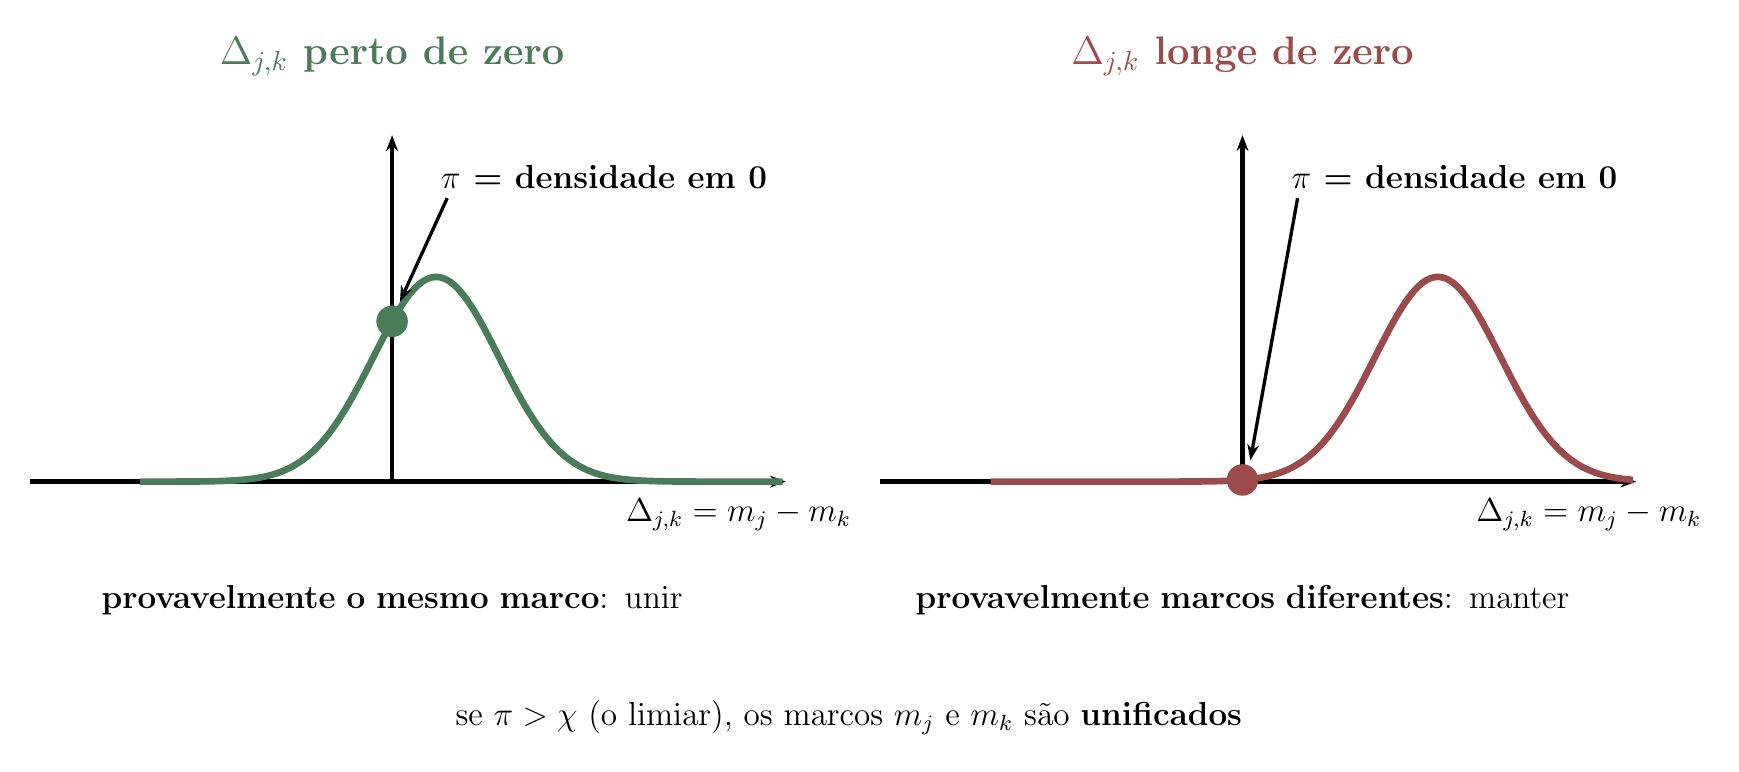
\begin{tikzpicture}[x=1cm,y=1cm]
\foreach \o/\mu/\col/\tit/\res in {0/0.7/dgreen/{$\Delta_{j,k}$ perto de zero}/{\textbf{provavelmente o mesmo marco}: unir}, 10.8/3.1/dred/{$\Delta_{j,k}$ longe de zero}/{\textbf{provavelmente marcos diferentes}: manter}} {
  \node[font=\Large\bfseries, text=\col] at ({\o+4.2},5.4) {\tit};
  \draw[line width=1.6pt, ->] ({\o-0.4},0) -- ({\o+9.2},0);
  \draw[line width=1.6pt, ->] ({\o+4.2},0) -- ({\o+4.2},4.4);
  \node[font=\large, anchor=north] at ({\o+8.6},-0.1) {$\Delta_{j,k}=m_j-m_k$};
  \draw[domain=-4.0:6.2, samples=90, smooth, line width=2.4pt, draw=\col] plot ({\o+4.2+\x*0.8},{2.6*exp(-0.5*((\x-\mu)/1.0)^2)});
  \fill[\col] ({\o+4.2},{2.6*exp(-0.5*(\mu)^2)}) circle (0.2);
  \draw[->, line width=1.2pt] ({\o+4.9},3.6) -- ({\o+4.3},{2.6*exp(-0.5*(\mu)^2)+0.25});
  \node[font=\large\bfseries, anchor=south west] at ({\o+4.7},3.6) {$\pi$ = densidade em 0};
  \node[font=\large, text width=9cm, align=center] at ({\o+4.2},-1.5) {\res};}
\node[font=\large, text width=19cm, align=center] at (10.0,-3.0) {se \mbox{$\pi>\chi$} (o limiar), os marcos $m_j$ e $m_k$ são \textbf{unificados}};
\end{tikzpicture}
\end{document}
